\documentclass[11pt,a4paper]{article}
\usepackage[T1]{fontenc}
\usepackage[utf8]{inputenc}
\usepackage{lmodern}
\usepackage[margin=2.35cm]{geometry}
\usepackage{setspace}
\setstretch{1.05}
\usepackage{amsmath,amssymb,booktabs}
\usepackage{graphicx}
\usepackage{siunitx}
\sisetup{detect-weight=true,detect-family=true}
\DeclareSIUnit{\ppb}{ppb}
\usepackage[numbers,sort&compress]{natbib}
\usepackage{microtype}
\usepackage{caption}
\captionsetup{font=small,skip=4pt}
\usepackage[hidelinks]{hyperref}
\setlength{\parskip}{0.28em}
\setlength{\parindent}{1.05em}

\title{Three-Valve Nonlinear Model Predictive Control\\ for High-Gravity Beer Blending}
\author{Department of Computer Science}
\date{October 2026}

\begin{document}
\maketitle
\begin{abstract}
\noindent
High-gravity blending dilutes a concentrated mother beer with cold deaerated water. The actuators are three control valves---beer, dilution water, and the line leaving the skid---and a carbon-dioxide injector. Industrial practice closes a flow ratio and a separate pressure loop. That station can hold a quiet point. It does not plan a brand change, and it has no prediction of the pressure at which carbon dioxide leaves solution inside a valve. This paper puts the three lifts and the carbon-dioxide dose in one nonlinear model predictive program. Original extract is the Balling map, so extract and alcohol are not treated as two linear dilutions of one ratio. The throat pressure of each valve is required to stay above the composition-dependent equilibrium pressure. On an \SI{80}{\litre} mixer at \SI{20}{\cubic\metre\per\hour}, the controller, given a commissioned hydraulic model, brings a lager-to-light grade change inside \SI{0.05}{\degree}P in \SI{16}{\second}. The same program on a biased nominal model leaves an offset of about \SI{0.19}{\degree}P and matches a well-tuned ratio station on extract. When the mother beer cannot meet extract and alcohol together, the program returns the tolerance-weighted compromise.
\end{abstract}

\section{Introduction}
High-gravity brewing ferments a wort stronger than the beer that will be sold and restores sales strength by adding water \citep{stewart2010,kunze2019}. The blend skid is the step that sets original extract, alcohol and carbonation. Commercial frames quote tolerances of about \SI{0.05}{\degree}P and \SI{0.03}{\percent} by volume and implement them with ratio control \citep{centec2024,corosysweb}. Foam, yeast stress and flavour differences of the strong fermentation are upstream of this skid. Dissolved oxygen that arrives in the dilution water is likewise outside the authority of the valves. What the valves can still damage is the brand itself: a wrong ratio, or a throat pressure low enough to strip carbon dioxide.

The relative-gain array at the design point is diagonally dominant, so a decentralised pairing of beer lift with beer flow, water lift with water flow, and final lift with mix pressure is a fair steady-state station \citep{bristol1966,shinskey1996}. The difficulty is the transient and the output map. Original extract is not proportional to the mother-beer mass fraction. A ratio taken from original extracts misses the true extract by about \SI{0.19}{\degree}P, four times the release tolerance. Carbon dioxide equilibrium pressure depends on temperature, composition and concentration \citep{speers2013,rammert1991}. A pressure loop with a fixed setpoint does not follow that pressure when the brand changes.

Model predictive control is the standard way to move several constrained actuators against a nonlinear output map \citep{qin2003,rawlings2017}. Brewing applications have used it on fermentation temperature over days. The contribution here is the hydraulic program for this skid: three valve lifts and the carbon-dioxide dose, predicted with the Balling map and with the vena-contracta constraint written on carbon-dioxide equilibrium pressure rather than on the vapour pressure of water.

\section{Plant model}
Mother beer at the design point has alcohol \SI{5.40}{\percent} by weight, real extract \SI{6.10}{\percent} by weight, original extract \SI{16.319}{\degree}P and \SI{5.50}{\gram\per\litre} of carbon dioxide, at \SI{2}{\celsius}. Original extract of a blend is
\begin{equation}
p_{\mathrm{OE}}
=
\frac{100\,(2.0665\,A_w + E_r)}{100 + 1.0665\,A_w},
\label{eq:balling}
\end{equation}
with $A_w$ and $E_r$ in percent by weight \citep{kunze2019}. Alcohol by volume is $A_w\rho/789.24$. Both $A_w$ and $E_r$ scale with the mother-beer mass fraction $w$, and $p_{\mathrm{OE}}$ does not. The sales lager is $w=0.70$, hence \SI{11.613}{\degree}P and \SI{4.833}{\percent} by volume. The light brand is $w=0.58$, hence \SI{9.687}{\degree}P and \SI{4.000}{\percent} by volume. A linear dilution of the mother-beer original extract at the lager $w$ is already about \SI{0.19}{\degree}P off \eqref{eq:balling}'s value. The mass fraction that hits the Balling target is $0.70$, not the linear ratio.

Each valve is an equal-percentage trim of rangeability $50$ \citep{iec60534},
\begin{equation}
Q = K_v\,50^{\,l-1}\sqrt{\frac{\Delta p}{\rho/1000}}.
\end{equation}
Capacities are $32$, $12$ and $64$ cubic metres per hour. The mix pressure is the scalar unknown that matches mass flow into the mixer with the flow through the final valve after the blend-line loss. The throat pressure is $p_{\mathrm{vc}}=p_1-(p_1-p_2)/F_L^2$, with recovery factors $0.90$, $0.93$ and $0.86$. Carbon dioxide flashes if $p_{\mathrm{vc}}$ falls below $p_{\mathrm{eq}}=c/(\kappa_\zeta\zeta)$. At the lager point $p_{\mathrm{eq}}=\SI{1.905}{bar}$ absolute, the mix node is \SI{2.855}{bar}, and the final throat is \SI{2.279}{bar}. The mixer holds \SI{80}{\litre}. At \SI{20}{\cubic\metre\per\hour} its residence time is \SI{14.4}{\second}, which is the only slow time constant. Header pressures are \SI{4.80}{bar} on the beer, \SI{5.30}{bar} on the water and \SI{2.40}{bar} on the bright tank, all absolute.

\section{The predictive program}
Every \SI{4}{\second} the controller chooses two move blocks of $(l_h,l_w,l_f,\dot m_{\mathrm{CO_2}})$. Each block is held for three Euler steps of \SI{2}{\second}, so the horizon is \SI{12}{\second}, about $0.83$ residence times. The decision vector has length eight. Lifts stay in $[0.18,0.90]$, the dose in $[0,15]$ grams per second, and the lift may change by at most $0.16$ in one sample. The stage cost normalises each quality error by its tolerance,
\begin{equation}
\begin{aligned}
\ell
&=
\Big(\frac{p_{\mathrm{OE}}-p_{\mathrm{OE}}^{\star}}{0.05}\Big)^{2}
+
\Big(\frac{\mathrm{ABV}-\mathrm{ABV}^{\star}}{0.03}\Big)^{2}
+
\Big(\frac{c-c^{\star}}{0.05}\Big)^{2}\\
&\quad
+0.35\Big(\frac{Q_f-Q_f^{\star}}{0.5}\Big)^{2}
+
\text{soft pressure penalties}
+
\text{travel}.
\end{aligned}
\end{equation}
One tolerance of extract, alcohol or carbon dioxide costs $1$. A flow error of \SI{0.5}{\cubic\metre\per\hour} costs $0.35$. A throat or mix pressure inside the forbidden side of the margin is penalised at $6$ per bar squared, so a flash outranks a quality tolerance and a small pressure noise does not. The case-study solver is a warm-started sequential quadratic program with an iteration limit of six. A production implementation would replace those iterations by one real-time iteration \citep{diehl2005,rawlings2017}. The study does not impose a terminal constraint, and it does not claim a Lyapunov certificate \citep{mayne2000}.

The baseline is an incremental ratio station sized so that $K_I G_{ii}\Delta t$ is near $0.3$ on the diagonal gains \citep{skogestad2003}. Its pressure setpoint is fixed at the lager equilibrium plus \SI{0.90}{bar}. It inverts Balling for a feedforward mass fraction and trims extract with a slow integral. It cannot move the pressure setpoint when $p_{\mathrm{eq}}$ changes, and it cannot trade extract against alcohol when both targets are infeasible.

At the lager steady point the installed gains, in cubic metres per hour and bar per unit lift, are approximately
\begin{equation}
G
=
\begin{bmatrix}
48.05 & -3.21 & 7.64\\
-2.59 & 23.09 & 2.64\\
2.09 & 0.89 & -2.14
\end{bmatrix},
\end{equation}
and the relative-gain array is diagonally dominant with entries $0.87$, $0.95$ and $0.82$. Thirteen percent of the beer-flow relative gain sits on the final valve. That term is quiet at steady state and active during a grade change, which is why the three lifts are coordinates of one program.

\section{Numerical estimation}
The plant is a dynamic simulation, not a brewery trial. Sensor noise is shared across controllers. The outlet analysis is delayed \SI{12}{\second}; the mixer state used by the predictive controller is a flow integration. Three upsets are applied at $t=\SI{20}{\second}$.

On the grade change the commissioned model spends the whole rate limit on the first move: every lift changes by $0.16$. Beer flow falls from about \SI{13.8}{\cubic\metre\per\hour} to \SI{6.4}{\cubic\metre\per\hour} and water flow rises to about \SI{10.2}{\cubic\metre\per\hour}, so the inlet is lighter than the light brand. Extract error falls from \SI{1.92}{\degree}P to \SI{0.87}{\degree}P in four seconds. A pure residence-time decay of the same step would still be at \SI{1.46}{\degree}P. The error enters and remains inside \SI{0.05}{\degree}P at \SI{16}{\second}. The extract integral is \SI{10.75}{\degree}P$\cdot$s. The ratio station and the predictive controller on the nominal model finish at \SI{31.30}{\degree}P$\cdot$s and \SI{32.29}{\degree}P$\cdot$s, and neither enters the band. The nominal tail is $+\SI{0.19}{\degree}P$. Valve travel is about $1.7$ lift-units for both predictive controllers and $7.1$ for the ratio station, which reverses while the vessel is still exchanging. Figure~\ref{fig:s1} shows the three quality traces.

\begin{figure}[t]
\centering
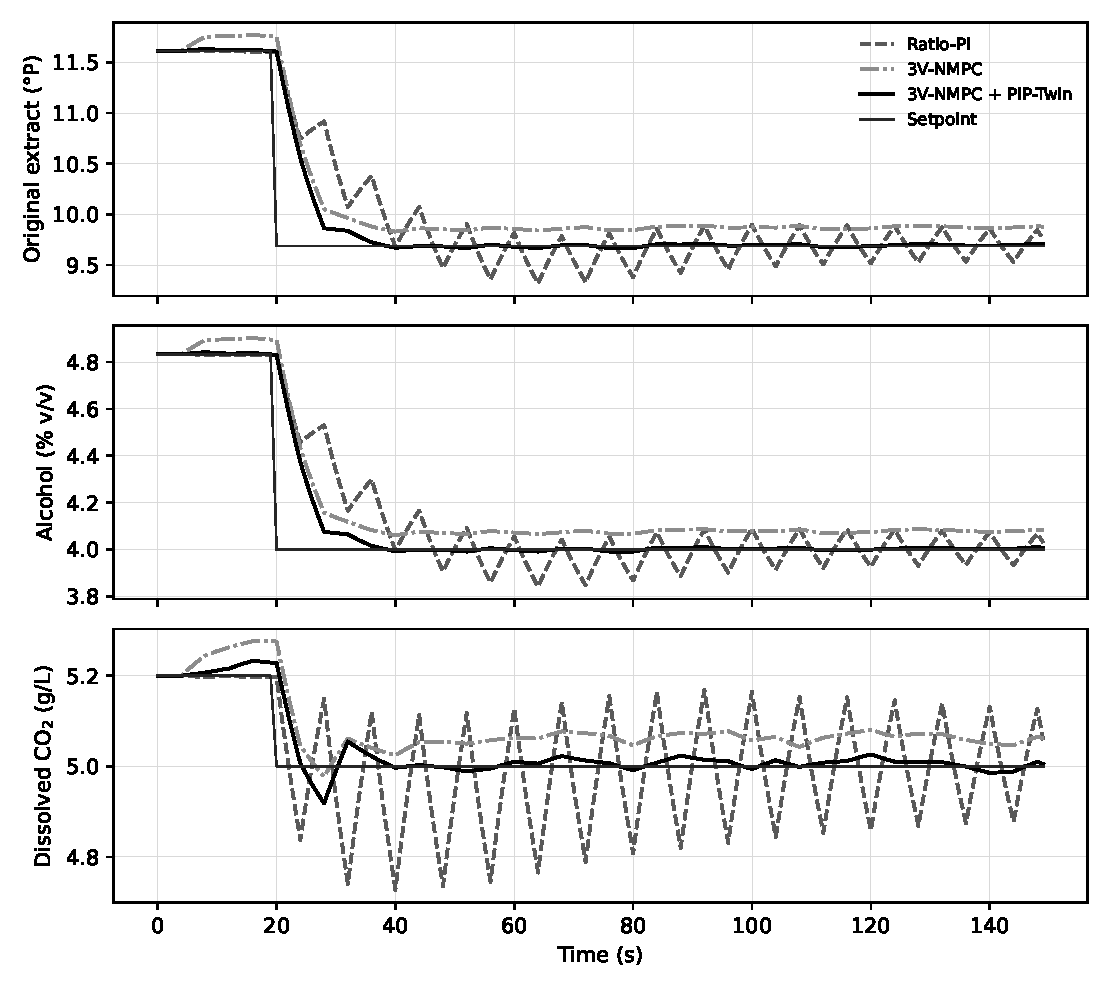
\includegraphics[width=0.86\textwidth]{../main/figures/s1_quality.pdf}
\caption{Original extract, alcohol and carbon dioxide on the lager-to-light grade change. The commissioned predictive controller is the solid trace.}
\label{fig:s1}
\end{figure}

\begin{table}[t]
\centering
\caption{Extract, alcohol and carbon-dioxide integrals from the upset to the end of each run. Settling time is the first instant after which the extract error remains inside \SI{0.05}{\degree}P.}
\label{tab:kpi}
\scriptsize
\setlength{\tabcolsep}{3.2pt}
\begin{tabular}{@{}llrrrr@{}}
\toprule
Case & Controller & IAE OE & IAE ABV & IAE CO$_2$ & Settle (s) \\
\midrule
Grade change & Ratio & 31.30 & 13.48 & 11.81 & 129 \\
Grade change & Nominal NMPC & 32.29 & 13.90 & 8.10 & 129 \\
Grade change & Commissioned NMPC & 10.75 & 4.63 & 2.06 & 16 \\
Infeasible mother beer & Ratio & 12.38 & 21.44 & 2.83 & 139 \\
Infeasible mother beer & Nominal NMPC & 39.34 & 9.96 & 5.06 & 139 \\
Infeasible mother beer & Commissioned NMPC & 20.04 & 17.80 & 1.27 & 139 \\
Oxygen and stiction & Ratio & 3.97 & 1.73 & 1.07 & 107 \\
Oxygen and stiction & Nominal NMPC & 19.28 & 8.41 & 6.06 & 116 \\
Oxygen and stiction & Commissioned NMPC & 1.29 & 0.56 & 0.95 & $<$1 \\
\bottomrule
\end{tabular}
\end{table}

The second upset makes the brand infeasible. Mother-beer real extract rises by $0.45$ percentage points and alcohol falls by $0.25$, and the beer header drops by \SI{0.45}{bar}. The mass fraction that minimises the tolerance cost is $w=0.712$, at \SI{11.780}{\degree}P and \SI{4.696}{\percent} by volume. The commissioned tail is \SI{11.777}{\degree}P and \SI{4.695}{\percent} by volume. The ratio station is extract-greedy. The nominal predictive controller chases alcohol, because its gain is wrong. No second ratio creates the missing alcohol.

The third upset raises dilution-water oxygen from \SI{12}{ppb} to \SI{85}{ppb} and sticks the water valve with a deadband of $0.03$ lift. Product oxygen reaches about \SI{31}{ppb} for every controller. The valves do not remove it. With the deadband inverted, the commissioned extract integral is \SI{1.29}{\degree}P$\cdot$s and the error never leaves the band. The nominal program, which does not know the stick, is the worst of the three stations on extract.

\section{Conclusion}
The innovation is the joint program: three lifts and the carbon-dioxide dose, a Balling output map, and a vena-contracta constraint written on carbon-dioxide equilibrium pressure. Decentralised ratio control remains a competent steady station. On a feasible grade change it is slow, and on an infeasible mother beer it spends the only ratio on extract. The predictive program returns the weighted compromise when both targets cannot be met, and it keeps the throat pressure above equilibrium at the design point used here. Those closed-loop numbers hold when the hydraulic model has been commissioned. On the nominal model the same program does not improve extract over the ratio station. The companion paper treats that commissioning problem. The study is a reproducible simulation of one skid. It is not a plant trial, and the short-horizon solver used here is not a certified real-time iteration.

\bibliographystyle{unsrtnat}
\bibliography{refs}
\end{document}
